\chapter{基本原理}
\newpage
\section{概要}
本章では, 本研究で具体的な焦点となる超音波の性質, エラストグラフィーの原理, 超音波プローブについての基礎的な原理について示す.

\section{超音波とは}
超音波は, 人の可聴域を超える20kHz以上の高周波の音波である. 超音波は運輸, 製造業, 建築, 水道, 農林水産, 食品そして医療に至るまで様々な分野で利用されている. 医療分野では診断装置, センサ, 通信機器, 補助具, 溶着などで多用されている. 

\section{超音波の性質}
医療機器では1\verb|〜|20MHzの超音波を使用しており, 超音波が生体内を伝播することで伝播経路における音響特性が変化する. この音響特性の分布の変化を解析することで, 生体内の組織の状態を観測できる. 以下で, 超音波と生体組織をの関係を述べるにあたり, 必要となる超音波の基本的な性質について述べる[10].
\subsection{反射と屈折}
超音波は異なる屈折率をもつ2つの物質を通過する際に, その境界面で反射・屈折を起こす. \figref{hansha} に音速$c_0$, 密度$\rho_0$の媒質から, 音速$c_1$, 密度$\rho_1$の媒質に超音波が入射する様子を示す. $\theta_0$, $\theta_1$はそれぞれ入射角, 屈折角を表す, また, 音速の異なる媒質に入射する際, 超音波の一部は境界面で反射する. \figref{hansha}の$\theta_0^{\prime}$で表されているのが反射角である. 入射角と反射角は等しい. また, 入射波と透過波の間ではSnellの法則が成り立つ.
\begin{equation}
\\ \dfrac{\sin\theta_0}{c_0} = \dfrac{\sin\theta_1}{c_1}
\end{equation}
生体組織では, 様々な音響特性をもつ物質が存在するため, 超音波パルスを与えた際に観察される複雑な波形の乱れは, 生体組織の境界面や音響特性などをはじめとした生体組織を特徴付ける, 様々な情報を含んでいる. 
\begin{figure}[H]
  \begin{center}
    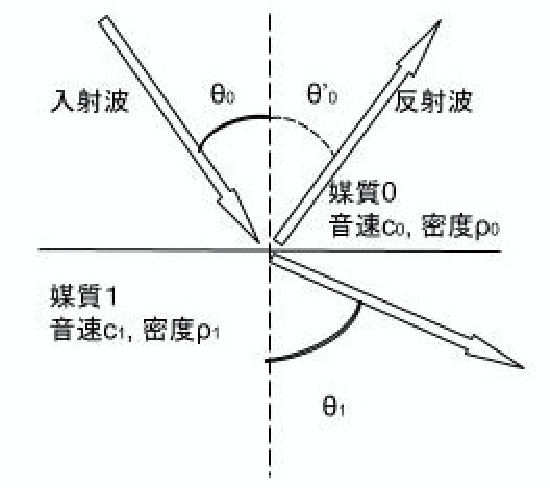
\includegraphics[width=75mm]{fig/hansha.pdf}
  \end{center}
  \caption{屈折率の異なる媒質間の境界面での超音波の挙動}
  \figlab{hansha}
\end{figure}
\subsection{音響インピーダンス}
音響インピーダンスとは, 音波の伝播に際する通りにくさを表し, 電気工学でいう所の抵抗$R$であるというアナロジー的な説明が成されることが多い. 音響インピーダンスは物質ごとに固有な値であり, 振動数や振幅とは独立である. 音響インピーダンスは, 物質の密度,物質固有の音速cを用いて以下の式で表せる.
\begin{equation}
\label{eq.impeadance}
\\ $Z$ = \rho \times $c$
\end{equation}
音響インピーダンスの差異が超音波の反射や屈折のような現象を引き起こす. \figref{impeadance} に示すように, 境界面に対して超音波が直角に入射した際も, 音響インピーダンスの差異によって, 反射波, 透過波が生じる. \figref{impeadance} に音響インピーダンス$Z_0$, 密度$\rho_0$, 音速$c_0$から音響インピーダンス$Z_1$, 密度$\rho_1$, 音速$c_1$へ超音波が入射する様子を示す. 連続の式より, 反射率Rと透過率Tはそれぞれ(\ref{eq.R})式および(\ref{eq.T})式のように示せる.
\begin{equation}
\label{eq.R}
\\$R$= \dfrac{Z_2 - Z_1}{Z_2 + Z_1}
\end{equation}
\begin{equation}
\label{eq.T}
\\$T$= \dfrac{2Z_2}{Z_2 + Z_1}
\end{equation}
人体では, 骨などの音響インピーダンスの大きい部分では反射が生じるので, 超音波CTで得られる断層画像にも大きな影響を及ぼす. 
\begin{figure}[H]
  \begin{center}
    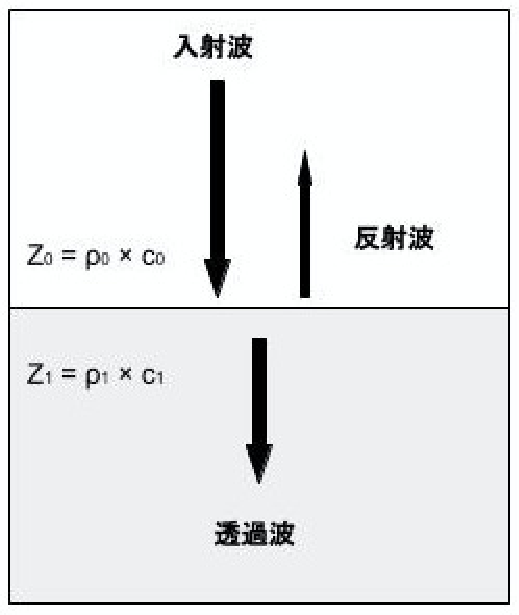
\includegraphics[width=75mm]{fig/impeadance.pdf}
  \end{center}
  \caption{音響インピーダンスの異なる媒質間の境界面での超音波の挙動}
  %[内閣府, 平成30年版高齢社会白書(全体版)]
  \figlab{impeadance}
\end{figure}
\subsection{音速と体積弾性率}
音速は媒質を物理的に振動させることによって, 媒質の粗密が媒質中を伝播していく時の速度である. 生体内で伝搬する超音波は縦波で, その伝搬速度$c$は体積弾性率$K$および平均密度$\rho$を用いて, (\ref{eq.c})式のように表せる.
\begin{equation}
\label{eq.c}
\\$c$\ = \sqrt{\dfrac{K}{\rho}}
\end{equation}
\subsection{散乱}
波長と同程度のサイズの媒質に入射すると回折が起こる. 生体内では, 反射, 屈折, 回折によって散乱が起こる. 波長に対して散乱体径が小さい場合は, 散乱強度は入射波の周波数の4乗に比例し, 光学におけるレイリー散乱のような振る舞いをする[11]. 波長と散乱体径が近い場合, ミー散乱に近い振る舞いをする. 
\subsection{減衰}
減衰は, 散乱と吸収によって2点を結ぶ直線経路間のエネルギーの損失を表す. 生体組織は音速や密度が不均一に分布するため, 上述したように, 反射, 屈折, 回折などの現象が複雑に作用することで散乱場が生じる. 散乱は超音波のエネルギー損失を引き起こさない. 一方, 吸収は伝播中に超音波のエネルギーが熱に変換され, 音響エネルギーを失う.
\\\ \ 減衰率$\alpha$は, 初期音圧$p_0$, 伝播距離$x$, 減衰後の音圧$p$を用いて(\ref{eq.alpha})式のように表される.
\begin{equation}
\label{eq.alpha}
\\\alpha = \frac{20}{x}  \log_{10} \frac{p_0}{p_1}
\end{equation}
生体内では, 減衰率$\alpha$は周波数$f$に依存し, 周波数$f$, 乗数$y$, 定数$\alpha_0$を用いて(\ref{eq.alpha_2})式のように表される.
\begin{equation}
\label{eq.alpha_2}
\\\alpha = \alpha_0f^y
\end{equation}
表\ref{table_soshiki}に, 人体の組織における減衰定数0と周波数fについてまとめる.

\begin{table}[htb]
\centering
\caption{人体の様々な組織における減衰率}
\label{table_soshiki}
\begin{tabular}{|c|c|c|}
\hline
組織 & 減衰率$\alpha_0$ & 計測周波数$f$[Hz]  \\ \hline
血液 & 0.2$\times$$10^{-7}$ &      1 \\ \hline
脳   & 1.05$\times$$10^{-7}$ &      3.4\\ \hline
肝臓  & 0.77$\times$$10^{-7}$ &     3 \\ \hline
脂肪 & 0.45$\times$$10^{-7}$ &     3.4 \\ \hline
頭蓋骨  & 24$\times$$10^{-7}$ &     1.8  \\ \hline
\end{tabular}
\end{table}

\section{エラストグラフィの原理}
医用画像の歴史は, ヴィルヘルム・コンラート・レントゲンの1895年のX線の発見にまで遡る. レントゲンは世界で初めてX線写真の撮影に成功したが,  生体にメスを入れることなく生体内部を可視化できることは, 非常に画期的なことであった. その後, 医用画像はディジタル計算機の登場により更に進化を遂げ, 今日ではX線画像だけでなく, 超音波画像, CT画像など医用画像の種類も多様化した. 超音波を用いた医用画像の取得は, 特にディジタル計算機の恩恵を受けた技術であり, 今後更なる発展が見込まれている. 以下では, エラストグラフィの原理について詳しく説明する. %[12].ここの引用はもう一度考えよう. 
%\begin{itemize}
\subsection{生体組織の弾性と粘性\cite{elastography2}}
生体組織はそれぞれの組織において様々な弾性と粘弾性を持っているため, 組織全体は不均一で複雑に入り組んだ構造となっている. そのため, 生体組織の力学的な挙動を記述する粘弾性モデルを仮定し, 弾性率を推定する.%https://www.jstage.jst.go.jp/article/mit/32/2/32_63/_pdf.
エラストグラフィでは, 組織を加圧あるいは加振することで粘性と弾性を評価し, 生体組織の硬さを計測する. 弾性を評価するにあたって, ヤング率は非常に重要なパラメータである. \figref{young}のように, 長軸方向に応力を加えたモデルを考える. 
\begin{figure}[H]
  \begin{center}
    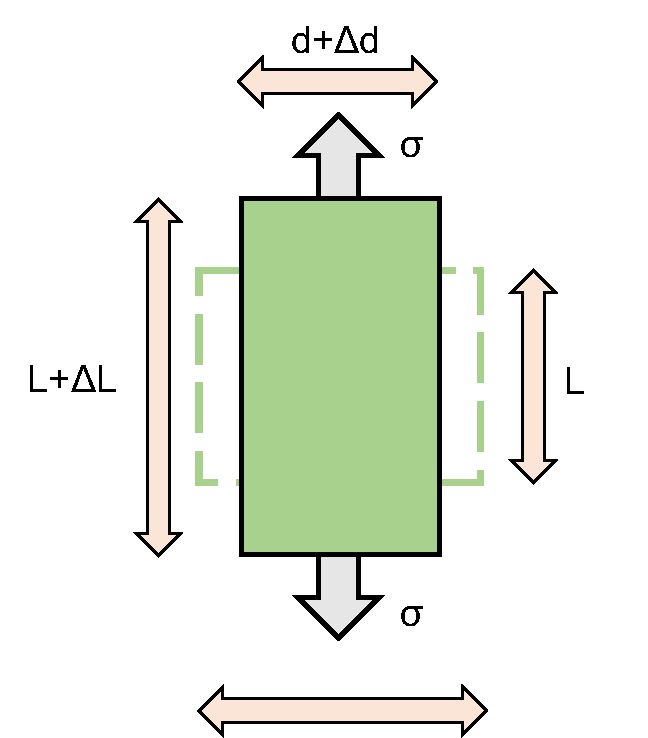
\includegraphics[width=60mm]{fig/young.pdf}
  \end{center}
  \caption{ヤング率と応力の関係}
  %[内閣府, 平成30年版高齢社会白書(全体版)]
  \figlab{young}
\end{figure}
フックの法則から応力$\sigma$と縦ひずみ$\epsilon$を用いて(\ref{eq.young})式のように表せる. 
\begin{equation}
\label{eq.young}
\\$E$ =  \dfrac{\sigma}{\epsilon}
\end{equation}
縦ひずみ$\epsilon$および, 横ひずみ$\epsilon_r$はそれぞれ(\ref{eq.tate})式および(\ref{eq.yoko})式のように定義される. 
\begin{equation}
\label{eq.tate}
\\\epsilon =  \dfrac{\Delta L}{L}
\end{equation}
\begin{equation}
\label{eq.yoko}
\\\epsilon_r =  \dfrac{\Delta d}{d}
\end{equation}
また, 剛性率およびポアソン比は(\ref{eq.gou})式および(\ref{eq.poa})式のように定義される. 
\begin{equation}
\label{eq.gou}
\\G =  \dfrac{\sigma_s}{\epsilon_s}
\end{equation}
\begin{equation}
\label{eq.poa}
\\\nu =  \dfrac{\epsilon_r}{\epsilon}
\end{equation}
ただし, $\sigma_s$はせん断応力, $\epsilon_s$はせん断ひずみとする. また, ヤング率$E$と剛性率$G$とポアソン比$\nu$との関係は(\ref{eq.egnu})式で表せる. 
\begin{equation}
\label{eq.egnu}
\\E=  2(\nu + 1)G
\end{equation}
ポアソン比は生体組織の部位によって異なるため, ヤング率と剛性率の関係もそれに応じて変化する. 
\\\ 次に粘性について説明する. 粘性率は$\mu$で表され, (\ref{eq.nensei})式のように応力とひずみ速度を記述できる. 
\begin{equation}
\label{eq.nensei}
\\\sigma =  \mu \dfrac{d \epsilon}{dt}
\end{equation}
%https://www.jstage.jst.go.jp/article/mit/32/2/32_63/_pdf
(\ref{eq.nensei})式から, 粘性の影響は生体組織に加える圧力や振動, 周波数に依存することがわかる.
\\\ 弾性率は波の伝搬速度を決める要素でもあり, パルスエコー法では縦波を用いる. 縦波は軟組織では1500m/sである. これに対し, せん断波はMHz帯域では生体内で激しく減衰するが, 1kHZ程度の大衆はでは伝搬可能である. 静的な変形においてはせん断波の速度$c_s$は(\ref{eq.sendan})式のように表せる.
\begin{equation}
\label{eq.sendan}
\\\ c_s = \sqrt{\dfrac{G}{\rho}}
\end{equation}
せん断波の速度$c_s$は1\verb|〜|10m/sであり, Gの値は1\verb|〜|100kPaと小さく, 組織間の違いが大きいという特徴がある. 
\\\ 一方, 動的な変形では波の伝搬の際に高周波では粘性の影響が無視できない. \figref{kelvin}はケルビン・フォークトモデルであり, 粘性を考慮したせん断波の速度は(\ref{eq.sendan})式の代わりに(\ref{eq.forkt})式で表せる. 
\begin{equation}
\label{eq.forkt}
\\\ c_s = \sqrt{\dfrac{2(G^2 + (2\pi \mu f)^2)}{\rho(G + \sqrt{G^2 + (2\pi \mu f)^2)}}}
\end{equation}
このように, 周波数$f$の関数になり, 高周波ほど速度が増加する. 
\begin{figure}[H]
  \begin{center}
    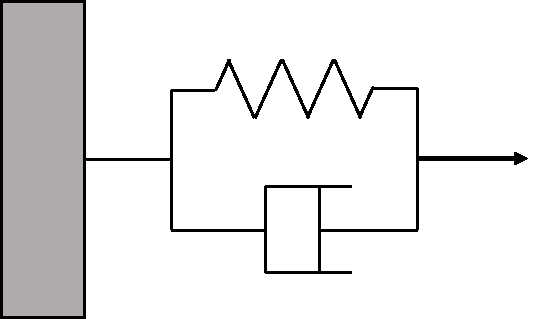
\includegraphics[width=60mm]{fig/forkt.pdf}
  \end{center}
  \caption{ケルビン・フォークトモデル}
  \figlab{kelvin}
\end{figure}
\subsection{超音波エラストグラフィの原理\cite{siina_2}}
軟組織の弾性の評価には, 大きく大別してストレイン・イメージングとシアウェーブ・イメージングの2つがある. 
\\\ ストレイン・エラストグラフィは外部から応力$\sigma$を与えて組織を変形させ, ひずみ$\epsilon$を測定する方法である. (\ref{eq.young})式よりヤング率を求める. この時, 体内での応力は一様であると仮定して, ひずみの分布を画像化する. 
\\\ シアウェーブ・イメージングは, 体内にせん断波を伝搬させ, その伝搬速度$c_s$を測定する. 媒質が非圧縮生で等方性があり, 密度$\rho$が既知であるとすれば(\ref{eq.egnu})式より$E$は(\ref{eq.3g})式で表せる. ただし, 軟組織ではポアソン比は約0.5であることを用いている. 
\begin{equation}
\label{eq.3g}
\\E=  3G = 3\rho c_s^2
\end{equation}
\ ストレイン・イメージングはプローブを用いてひずみの分布を画像化できるので, 簡便で実時間生が高く, Bモード像によるエコー信号を利用するので空間分解能も高いと言った利点がある. 一方で, ひずみは圧迫の強さに依存するので, 定性的な診断しかできない. また, 応力の分布が一様であると仮定しているため, 実際に応力が集中する部分ではひずみが大きくなり, 組織が実際より柔らかく表示されるアーチファクトが生じる. 腫瘍などの患部と周囲組織とのひずみの違いを画像化する際などに適用される. 
\\\ シアウェーブ・イメージングは音速を測定することで弾性率が求められるため, 定量生があるのが利点である. 一方でせん断波を生成する音響放射圧パルスの強さは, 通常の診断用の超音波よりも大きく, 多点の計測でそう照射エネルギーが大きくなる場合は, 計測の時間間隔を開ける必要があるため, 実時間性が低下する\cite{onkyouhousya}. 現在では, 伝搬方向を仮定して音速を求めるたが, これが原因でアーチファクトができる場合がある.
%\end{itemize}
\section{超音波プローブ}
超音波画像診断装置は, \figref{sindanblock}に示されるような構造をとる. プローブは, 対象物に超音波を送受信し, 対象物から得た物理的な振動を電気信号に変換することができる. 具体的には,\figref{probekouzou}で示されるように, プローブの内部構造は音響整合層, 音響レンズ, 圧電素子, パッキング材から成っている.  プローブの種類には主にコンベックス型, リニア型, セクタ型の3種類が用いられている(\figref{probesyurui}). それぞれのプローブの特徴を表\ref{table_probe}にまとめる. リニア型とセクタ型の欠点を補うようにしてコンベックス型ができた.本研究では, 前述した3種類のスキャン方法ではなく, Verasonicsと呼ばれるソフトウェアを利用した, 開口合成法というスキャン方法を用いる. 以下で開口合成法の原理について述べる. また, 開口合成法から得られたエコーデータの数値的な意味合いなどについても述べる. 
\begin{figure}[H]
  \begin{center}
    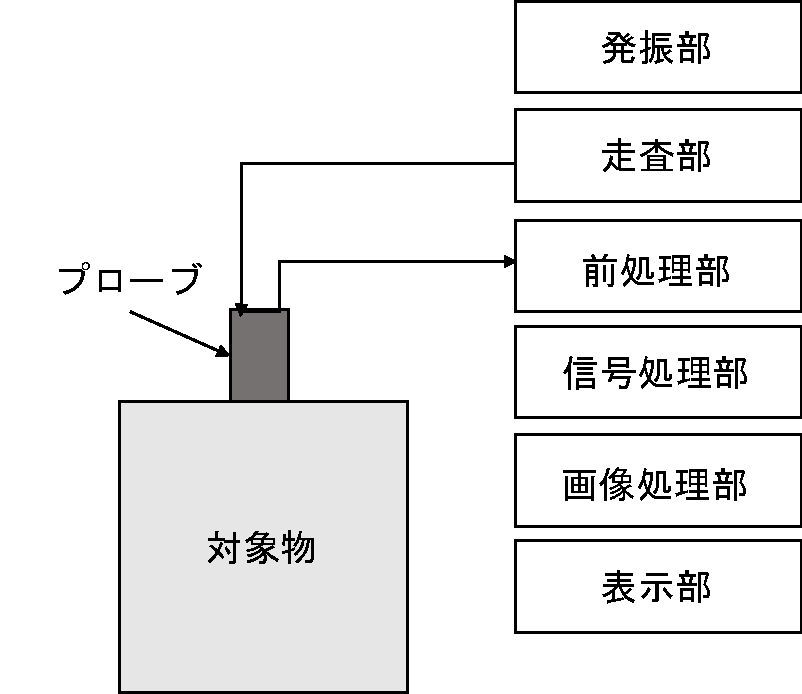
\includegraphics[width=60mm]{fig/ultradev.pdf}
  \end{center}
  \caption{超音波画像診断装置の概要}
  \figlab{sindanblock}
\end{figure}
\begin{figure}[H]
  \begin{center}
    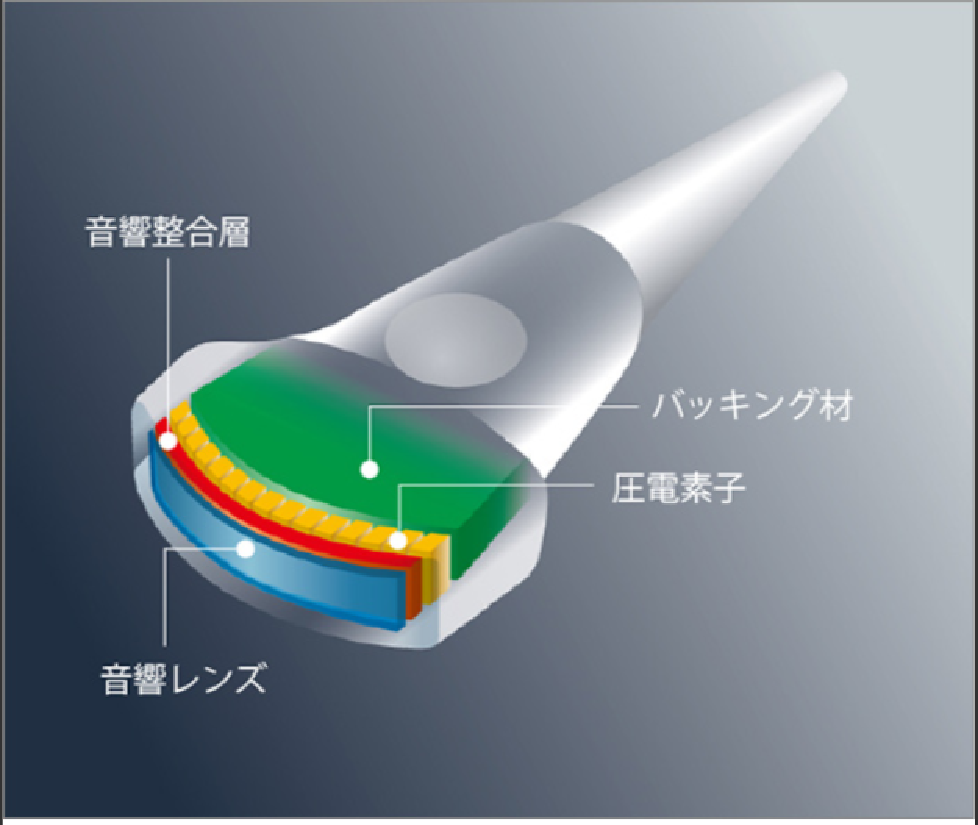
\includegraphics[width=60mm]{fig/img_probe.pdf}
  \end{center}
  \caption{プローブの構造}
  %http://www.yamauchi.co.jp/products/medical/probe.php
  \figlab{probekouzou}
\end{figure}
\begin{figure}[H]
  \begin{center}
    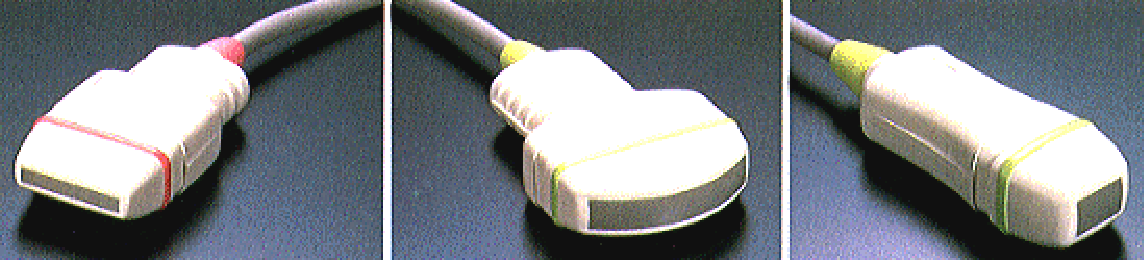
\includegraphics[width=100mm]{fig/probe3.pdf}
  \end{center}
  \caption{プローブの種類}
  %https://www.toshiba.co.jp/tech/review/1998/03/d06/fd06z3_j.htm
  \figlab{probesyurui}
\end{figure}

\begin{table}[htb]
\centering
\caption{プローブの特徴}
\label{table_probe}
\begin{tabular}{|c|p{3cm}|p{3cm}|p{3cm}|}%{|c|c|c|c|}
\hline
  &\hfil リニア型 \hfil & \hfil コンベックス型 \hfil & \hfil セクタ型 \hfil  
  \\ \hline
\hfil 適用箇所 \hfil &\hfil 関節/体表/腹部 \hfil & \hfil 腹部/臓器内 \hfil & \hfil 心臓/脳 \hfil    
\\ \hline
長所   & \hfil 生体内の組織構造を幅広く観察可能 \hfil & \hfil  深層部での広範囲にわたる観察が可能 \hfil & \hfil 深層部での広い視野での観察が可能 \hfil
 \\ \hline
短所  & \hfil 深層部では画像の解像度が低下する\hfil &\hfil  - \hfil& \hfil 浅部での視野が狭い \hfil \\ \hline
\end{tabular}
\end{table}
\subsection{開口合成法}
本研究では, プローブの超音波の送受信方法として, Verasonicsを用いてデータ取得を行うが, 中でも開口合成法を用いて実験系でのエコーデータを得る. Verasonicsの詳しい説明については, 第4章(%ページ数を書く)
で後述する. 開口合成法とは, 全素子の中から1つだけ送信素子を決め, そのほかのすべての素子を受信素子としてエコーデータを得る手法である. 送信素子の送波の時間間隔を適切に設定することで, 送信素子同士の干渉を無視できる. 開口合成法で得られたエコーデータは, リニア型, セクタ型のスキャンを擬似的にシミュレーションができるようにデータの並び替えが可能である.そのため, 開口合成法で得たデータから実験系に対して多角的な評価が可能にあると言う利点がある. このような利点から, 本研究では開口合成法で対象物をスキャンできるようにVerasonicsでプログラムを作成する. 
\begin{figure}[H]
  \begin{center}
    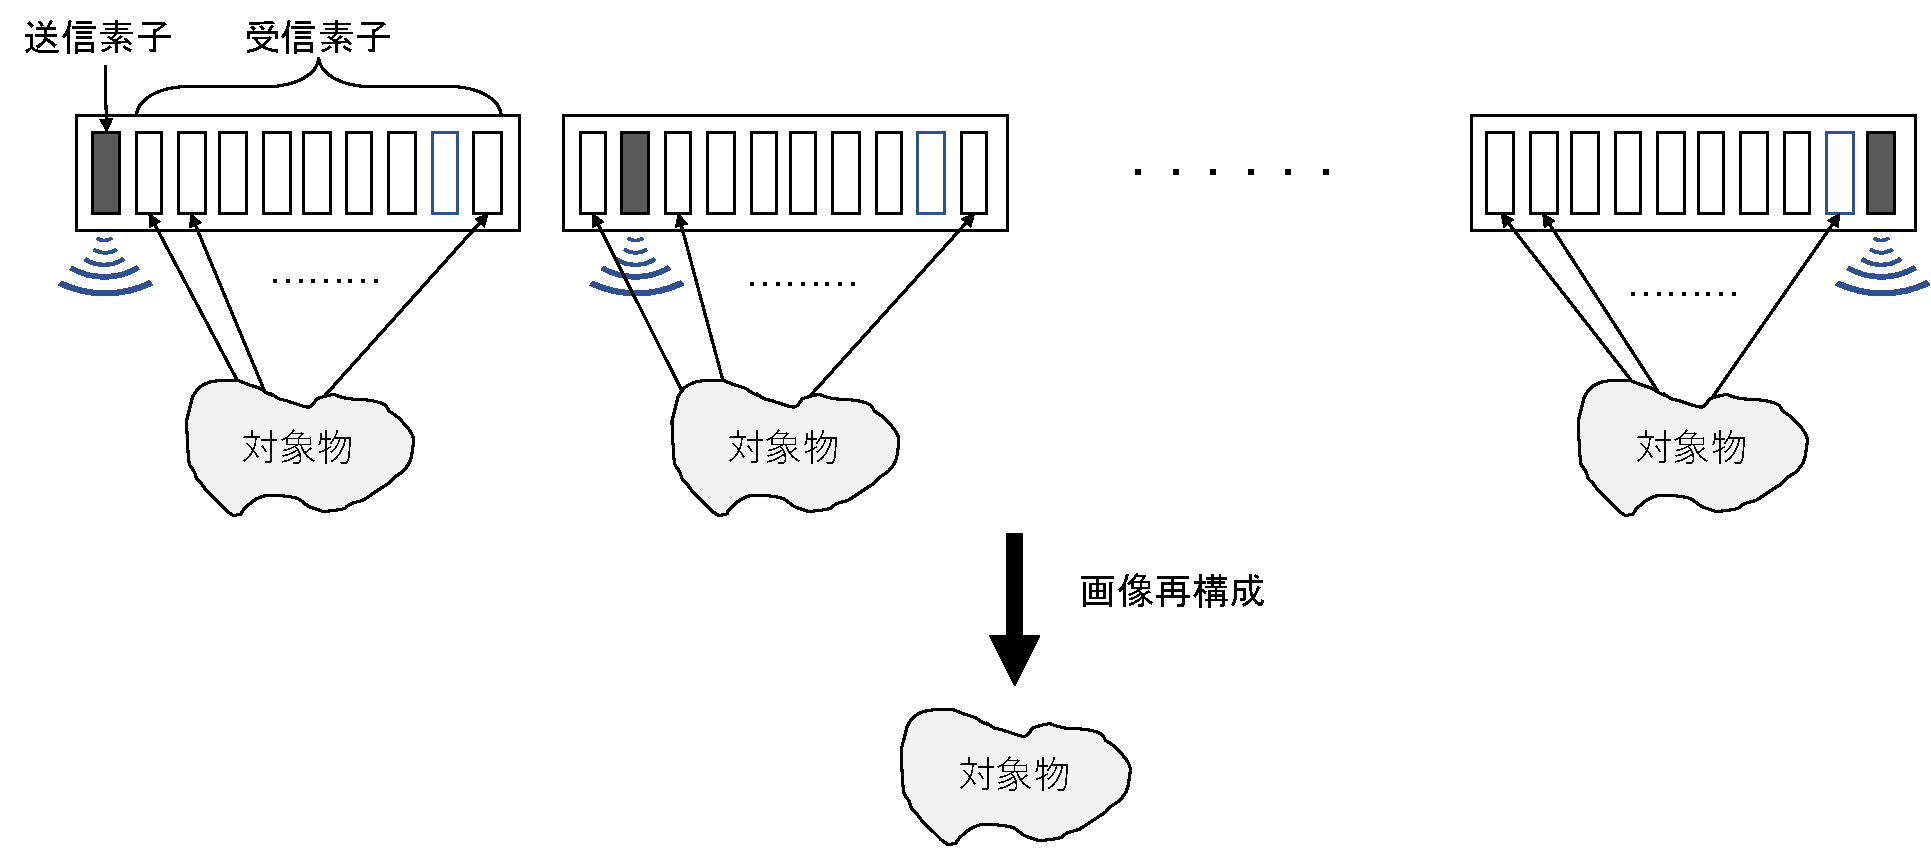
\includegraphics[width=140mm]{fig/kaikougousei.pdf}
  \end{center}
  \caption{開口合成法の概要}
  \figlab{kaikougousei}
\end{figure}
\subsection{エコーデータ\label{echodata}}
エコーデータとは, プローブの送信素子から送波された波が対象物で反射して受信素子に戻ってくる際の, 時間領域に対する音圧のデータのことである. 本研究ではVerasonicsから得られたエコーデータのことを以後RcvDataと呼ぶ. \figref{RcvData}は, リニア型のスキャンで得たRcvDataの例である. \figref{RcvData}および, \figref{RcvData_light}で示した例における, RcvDataの送信素子は64, 受信素子は256とする. RcvDataは(サンプリング数)×(受信素子番号)×(送信素子番号)のRF信号のデータ配列を持つ. RF信号とは, 高周波の信号のことである. \figref{RcvData}では, 32番目の送信素子から超音波を送波し, 32番目の受信素子でRF信号を得た際のRcvDataである. 横軸はサンプリング数であり, 時間軸に相当する. 縦軸は音圧である. 
\begin{figure}[H]
  \begin{center}
    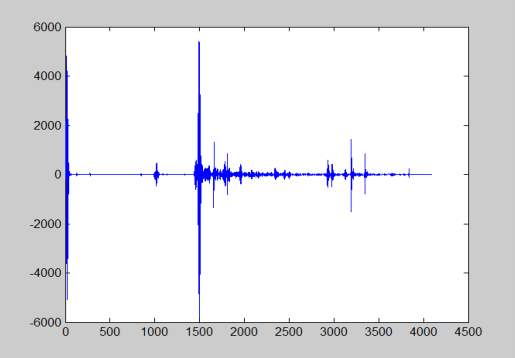
\includegraphics[width=65mm]{fig/RcvData_32.pdf}
  \end{center}
  \caption{RcvDataの例}
  \figlab{RcvData}
\end{figure}
\figref{RcvData_light}は, 32番目の送信素子に対する全受信素子数を横軸にとった際のRF信号を輝度表示したものである, ただし縦軸は時間軸に相当する. RF信号の値を足し合わせることで, 散乱体の反射強度をマッピングすることができる. 全送信素子に対してRF信号を足し合わせることで, 散乱体の位置を可視化する. さらに, RF信号のデータ配列をデシベル換算することで, \figref{RcvData_deci}を得る. この際, 輝度値は(\ref{eq.deci})式で計算できる. ただし, $I$は信号強度を, $E$は輝度値を表す. 
\begin{figure}[h]
  \begin{center}
    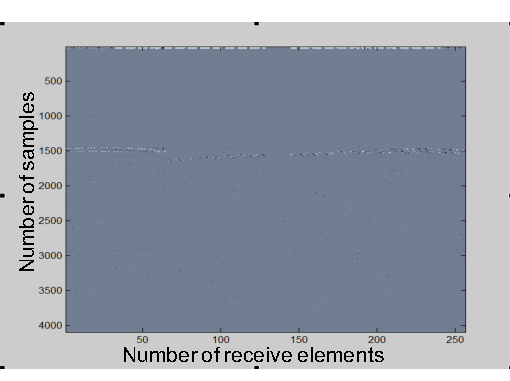
\includegraphics[width=65mm]{fig/RcvData_light.pdf}
  \end{center}
  \caption{RcvDataの輝度表示}
  \figlab{RcvData_light}
\end{figure}
\begin{equation}
\label{eq.deci}
\\\ E =20 \log_{10} I
\end{equation}
\begin{figure}[h]
  \begin{center}
    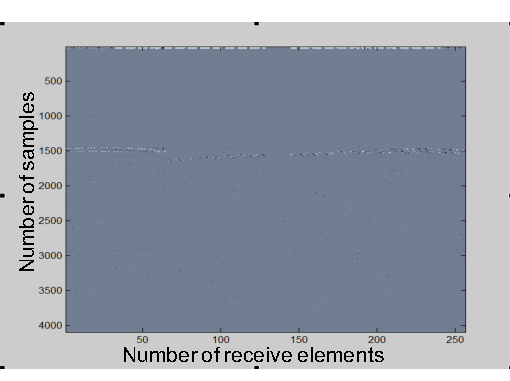
\includegraphics[width=65mm]{fig/RcvData_light.pdf}
  \end{center}
  \caption{RcvDataの輝度表示}
  \figlab{RcvData_deci}
\end{figure}
\subsection{エコーデータの信号処理}
第\ref{echodata}項で述べた通り, Verasonicsではプローブから得たエコーデータをRF信号として処理する. RF信号はまず, 同調回路により特定の周波数帯のみの信号を選択的に採用し, その後プローブの中心周波数に応じて周波数帯でRF信号をRF増幅器で増幅させる. 
\\\ \ 超音波画像診断装置では, プローブからの得たRF信号のうち時間ごとの振幅を主に信号情報として処理する. 振幅変調波のうち, 搬送波の信号を取り除き, 変調波の信号を取り出す復調処理を包絡線検波と呼ぶ %ちょい真似(竹内さん)
(\figref{hourakusen}). \figref{hourakusen}で示した, オレンジ色の曲線が包絡線に相当し, 変調波と呼ばれる. 緑色の波は搬送波と呼ぶ. 
\begin{figure}[h]
  \begin{center}
    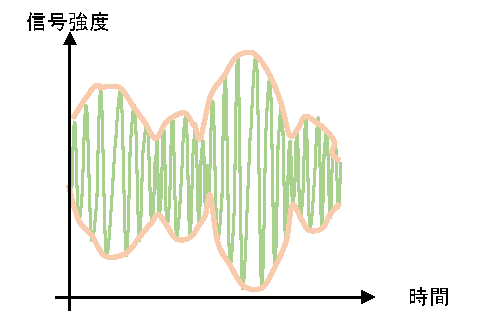
\includegraphics[width=65mm]{fig/hourakusen.pdf}
  \end{center}
  \caption{包絡線検波の概要}
  \figlab{hourakusen}
\end{figure}
\subsection{生体組織のひずみの測定}
本研究では, 振動モータで筋肉や腱を模した弦ファントムの他端を振動させ, その際の弦ファントムのひずみの伝搬を超音波画像診断装置のプローブで測定する. 第\ref{devicesection}章で, 実験装置の詳しい説明を行う. ファントムのひずみは, RFデータを処理することで算出できる. 
\\\ \ ファントムは振動モータによって振動するため, RFデータで隣接するフレームには微小な差異が生じる. したがって, 隣接するフレームの波形の移動量からファントムのひずみの伝搬が算出できる. フレームごとのRFデータの波形の類似度を測る手法として, SSD(Sum of Squared Difference), SAD(Sum of Absolute Difference), NCC(Normalized Cross-Correlation)がある. それぞれの類似度は, (\ref{eq.ssd})式\verb|〜|(\ref{eq.ncc})式で表せる\cite{yoshimurasan}. 
\begin{equation}
\label{eq.ssd}
\\\ R_{SSD} (t) =\sum_{n=u}^{u+W-1} [f(n) - g(n + t)]^2
\end{equation}
\begin{equation}
\label{eq.sad}
\\\  R_{SAD} (t) =\sum_{n=u}^{u+W-1} |f(n) - g(n + t)|
\end{equation}
\begin{equation}
\label{eq.ncc}
\\\ R_{NCC} = \dfrac{\sum_{n=u}^{u+W-1} f(n) * g(n + t)}{\sqrt{[\sum_{n=u}^{u+W-1}|f(n)|^2][\sum_{n=u}^{u+W-1}|g(n+t)|^2]}}
\end{equation}
SSDおよびSADは, サンプル点数の増加に伴い計算コストが高まる. 一方, NCCでは
